% !TEX encoding = UTF-8
% !TEX TS-program = pdflatex
% !TEX root = ../tesi.tex

\chapter{Fast Broadcast}
	Fast Broadcast \cite{4199282} is a multi-hop routing protocol for vehicular communication. Its main feature consists in breaking the assumption that all vehicles should know, a priori, their fixed and constant transmission range. This assumption is often unreasonable, especially in \acrshort{vaneta}s and urban environments, where electromagnetic interferences and obstacles such as buildings heavily influence the transmission range.
	
	
	Fast Broadcast employs two different phases:
	\begin{enumerate}
		\item the \textbf{Estimation Phase}, during which cars estimate their frontward and backward transmission range;
		\item the \textbf{Broadcasts Phase}, during which a car sends an Alert Message and the other cars need to forward it in order to propagate the information.
	\end{enumerate}

	\section{Estimation Phase}
		During this phase, cars try to estimate their frontward and backward transmission range by the means of Hello Messages. These beacons are sent periodically via broadcast to all the neighbors of a vehicle.
		
		
		Time is divided into turns and, in order to keep estimations fresh, data collected during a certain turn is kept for the duration of the next turn, then discarded. The parameter \textit{turnSize} specifies the duration of a turn: the authors suggest a duration of one second. A bigger \textit{turnSize} could guarantee less collisions to the detriment of freshness of information. On the other hand, the effects of a smaller \textit{turnSize} are specular to those just presented. 
		
		
		Using this approach, vehicles can estimate two different values:
		\begin{itemize}
			\item \textit{Current-turn Maximum Front Range (CMFR)}, which estimates the maximum frontward distance from which another car can be heard by the considered one;
			\item \textit{Current-turn Maximum Back Range} (CMBR), which estimates the maximum backward distance at which the considered car can be heard.
		\end{itemize}
		When the turn expires, the value of these variables is stored in the LMFR and LMBR variables (\textit{Latest-turn Maximum Front Range} and \textit{Latest-turn Maximum Back Range}, respectively). The algorithm uses both last turn and current turn data because the former guarantees values calculated with a larger pool of Hello Messages, while the latter considers fresher information.
		
		When sending a Hello Message (Algorithm \ref{alg:hello-message-sending}), the vehicle initially waits for a random time between 0 and \textit{turnSize}. After this, if it has not heard another Hello Message or a collision, it proceeds to transmit a Hello Message containing the estimation of its frontward transmission range.
		
		
		When receiving a Hello Message (Algorithm \ref{alg:hello-message-receiving}), the vehicle retrieves its position and the sender's position, calculates the distance between these two positions and then updates the CMFR field if the message comes from ahead, otherwise CMBR is updated. The new value is obtained as the maximum between the old CMFR or CMBR value, the distance between the vehicle and the sender, and the sender's transmission range estimation included in the Hello Message.
		
		\begin{algorithm}[H]
			\begin{algorithmic}[1]
				\ForEach{turn}
					\State sendingTime $\gets$ random(turnSize)
					\State wait(sendingTime)
					\If{$\neg$ (heardHelloMsg() $\lor$ heardCollision())}
						\State helloMsg.declaredMaxRange $\gets$ max(LMFR, CMFR)
						\State transmit(helloMsg)
					\EndIf
				\EndFor
			\end{algorithmic}
			\caption{Hello message sending procedure}
			\label{alg:hello-message-sending}
		\end{algorithm}
		
		\begin{algorithm}[H]
			\begin{algorithmic}[1]
				\State mp $\gets$ myPosition()
				\State sp $\gets$ helloMsg.senderPosition
				\State drm $\gets$ helloMsg.declaredMaxRange
				\State d $\gets$ distance(mp, sp)
				\If{receivedFromFront(helloMsg)} 
				\State CMFR $\gets$ max(CMFR, d, drm)
				\Else
				\State CMBR $\gets$ max(CMBR, d, drm)
				\EndIf
			\end{algorithmic}
			\caption{Hello message receiving procedure}
			\label{alg:hello-message-receiving}
		\end{algorithm}
	
	\section{Broadcast Phase}
		This phase is activated once a car sends an Alert Message. The other cars can exploit the estimation of transmission ranges to reduce redundancy in message broadcast. Each vehicle can exploit this information to assign itself a forwarding priority inversely proportional to the relative distance: the higher the relative distance, the higher the priority.  
		
		
		When the Broadcast Phase is activated , a vehicle sends an Alert Message with application specific data. Broadcast specific data is also piggybacked on the Alert Message, such as:
		\begin{itemize}
			\item \textit{MaxRange:} the maximum range a transmission is expected to travel backward before the signal becomes too weak to be received. This value is utilized by following vehicles to rank their forwarding priority;
			\item \textit{SenderPosition}: the coordinates of the sender.
		\end{itemize}
		Upon reception, each vehicle waits for a random time called \textit{Contention Window} (\textit{CW}). This window ranges from a minimum value (\textit{CWMin}) and a maximum one (\textit{CWMax}) depending on sending/forwarding car distance (\textit{Distance}) and on the estimated transmission range (\textit{MaxRange}), according to formula \ref{eq:contention-window}. It is quite easy to see that the higher the sender/forwarder distance is, the lower the contention window is.
		\begin{gather}
			\left\lfloor \left( \frac{\text{MaxRange} - \text{Distance}}{\text{MaxRange}} \times (\text{CWMax} - \text{CWMin}) \right) + \text{CWmin}  \right\rfloor
			\label{eq:contention-window}
		\end{gather}
		If another forwarding of the same message coming from behind is heard during waiting time, the vehicle suppresses its transmission because the message has already been forwarded by another vehicle further back in the column. On the contrary, if the same message is heard coming from the front, the procedure is restarted using the new parameters. The vehicle can forward the message only if the waiting time expires without having received the same message.
		
		Algorithm \ref{alg:alert-message-generation} and \ref{alg:alert-message-forwarding} describe the logic behind the Broadcast Phase.
		
		\begin{algorithm}[H]
			\begin{algorithmic}[1]
				\State alertMessage.maxRange $\gets$ max(LMBR, CMBR)
				\State alertMessage.position $\gets$ retrievePosition()
				\State transmit(alertMessage) $\gets$ helloMsg.declaredMaxRange
			\end{algorithmic}
			\caption{Alert Message generation procedure}
			\label{alg:alert-message-generation}
		\end{algorithm}
	
		\begin{algorithm}[H]
			\begin{algorithmic}[1]
				\State cwnd $\gets$ computeCwnd()
				\State waitTime $\gets$ retrievePosition()
				\State wait(waitTime
				\If{sameBroadcastHeardFromBack()}
				\State exit()
				\ElsIf{sameBroadcastHeardFromFront()}
				\State restartBroadcastProcedure()
				\Else 
				\State maxRange $\gets$ max(LMBR, CMBR)
				\EndIf 
			\end{algorithmic}
			\caption{Alert Message generation procedure}
			\label{alg:alert-message-forwarding}
		\end{algorithm}
	
	\section{Two dimensions extension}
		The original work \cite{4199282} considered only a strip-shaped road, where it was easy to define directions and establish 	when a message came from the front or the back. In \cite{BAR2017} an extension considering two dimensions was proposed. 
		
		
		The modifications to the Fast Broadcast algorithm are the following:
		\begin{enumerate}
			\item Utilizing only one parameter between CMBR and CMFR (thus considering only CMR):
			\item Including the position of the vehicle which originally generated the Alert Message in addition to the position of the sender of the message.
		\end{enumerate}
		
		
		When a vehicle receives an Alert Message, the origin-vehicle distance is confronted with the origin-sender distance: the vehicle can forward the message only if the former is greater than or equal to the latter, otherwise it simply discards the message.
		
		\begin{figure}[H]
			\centering
			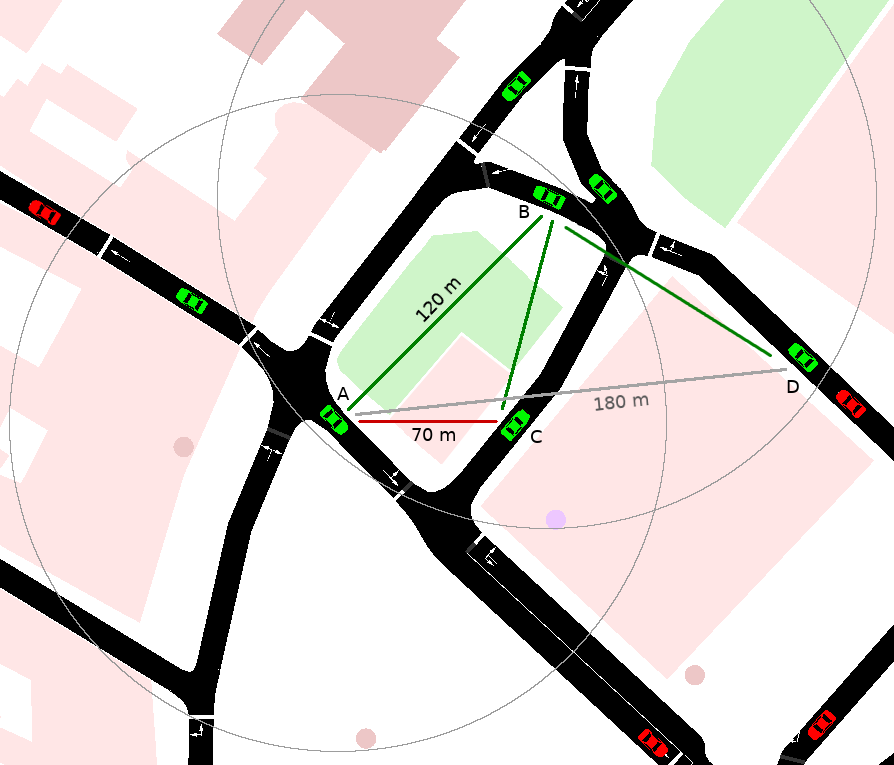
\includegraphics[width=\textwidth]{immagini/fb-2dpicc}
			\caption{Example of Fast Broadcast in 2d scenario}
			\label{fig:fb-2d}
		\end{figure}
		
		
		
		For example, suppose that vehicle A is the origin of the Alert Message and B receives it, but C doesn't due to an obstacle in the line of sight. B computes origin-vehicle distance, $d(A, B)$, and origin-sender distance, $d(A, A)$, which in this case are respectively 120 and 0m. Since origin-vehicle is greater than origin-sender, B can forward the Alert Message.
		
		
		Now suppose that C receives the message from B. C computes origin-vehicle distance, $d(A, C)$, and origin-sender distance, $d(A, B)$, which amount to 70 and 120m respectively. Since the former is not greater than or equal to the latter, C is not a candidate for forwarding and suppresses the transmission.
		
		
		D receives the message from B as well. D is a good candidate for transmission since the origin-vehicle distance, which amounts to 180m, is greater than origin-sender distance, equal to 120m.

%\chapter{L'offerta di \textit{stage}}
%\label{cap:loffertadistage}
%
%\section{\textit{Stage} in IBC: motivazioni aziendali}
%	\label{sec:motivazioni_aziendali}
%	IBC è un'azienda che in passato ha già offerto rapporti di \textit{stage}, anche se questo è il primo anno che essa partecipa a StageIt. Per non essere una perdita di tempo e risorse aziendali, gli \textit{stage} in IBC devono avere obiettivi e motivazioni che portano vantaggi anche a quest'ultima, oltre che allo stagista.
%	
%	\begin{itemize}
%		\item Il primo obiettivo che l'azienda tenta di raggiungere è lo studio di nuove tecnologie per andare ad espandere (e in alcuni casi sostituire) gli strumenti utilizzati. I dipendenti di IBC infatti sono quasi sempre impegnati in progetti con scadenze stringenti, il che rende molto difficile dedicare risorse alla scoperta e all'apprendimento di nuove tecnologie. Questi compiti sarebbero solitamente svolti dal reparto ricerca e sviluppo, assente in IBC. Le attività svolte durante lo \textit{stage} coprono quindi in parte questa mancanza, permettendo all'azienda di ottenere informazioni su nuovi strumenti e \gls{proofofconcept} di prodotti di futura realizzazione.
%		
%		
%		\item Il secondo obiettivo riguarda la prospettiva di assunzione di nuovo personale. L'azienda infatti tratta lo \textit{stage} come periodo di prova pre-assunzione, in modo da poter verificare le capacità dello stagista e fargli apprendere i meccanismi aziendali. IBC, al momento dell'offerta, era alla ricerca di programmatori Java e ha presentato una proposta proprio in quell'ambito. Assumere il tirocinante nello stesso ambito alla fine dello \textit{stage} fa risparmiare all'azienda tempo e risorse rispetto a un ulteriore addestramento in un'altra area.
%		
%		
%		\item La terza e ultima motivazione è il vantaggio che IBC può ottenere da una mente giovane e creativa, come ad esempio quella di uno studente che sta per concludere una laurea triennale in Informatica. Al contrario del personale abituato da anni a portare a termine gli stessi compiti nella stessa maniera, uno studente è più propenso ad inventare soluzioni originali e talvolta non convenzionali. Non sempre è detto che tali soluzioni siano adottabili e manutenibili, quindi è necessaria una revisione da parte di personale esperto prima che l'azienda adotti le proposte dello stagista.
%	\end{itemize}
%
%\section{Il progetto}
%
%	\subsection{Dominio applicativo}
%		Il progetto di \textit{stage} riguardava la memorizzazione di informazioni di prodotti commerciali. Il continuo rapporto con clienti in ambito \gls{retail} da parte di IBC porta alla necessità di avere una persistenza delle informazioni dei prodotti che essi offrono sul mercato. 
%		
%		\begin{figure}[H]
%			\centering
%			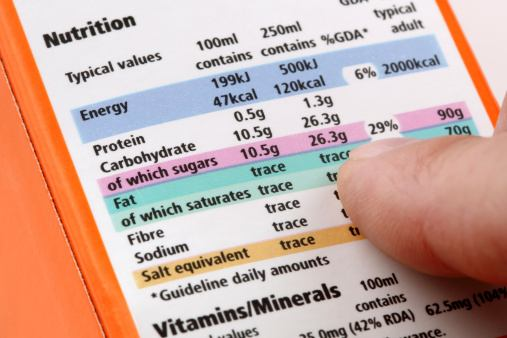
\includegraphics[scale=0.5]{immagini/etichetta}
%			\caption{Informazioni di un prodotto (\url{goo.gl/pxeYU1}).}
%		\end{figure}
%		
%		Questi dati sono utilizzati in molti ambiti, come ad esempio:
%		\begin{itemize}
%			\item La stampa dell'etichetta da apporre sulla confezione di un prodotto.
%			\item La categorizzazione di tipologie di prodotto sugli scaffali di un supermercato o sul sito di un \textit{e-commerce}.
%			\item L'identificazione e la ricerca di prodotti con particolari caratteristiche.
%			\item La gestione di magazzino.
%			\item L'identificazione di allergeni o particolari agenti chimici.
%			\item La raccolta di dati statistici e la generazione di reportistica.
%		\end{itemize}
%		
%		Dati i molti utilizzi, la memorizzazione delle informazioni è una necessità che negli anni ha avuto varie soluzioni e implementazioni.
%						
%		Attualmente IBC utilizza un \textit{database} relazionale per la persistenza dei dati. Questo porta al problema principale che il progetto offerto deve risolvere. Data la natura stessa del modello relazionale, è necessario definire una struttura prima di poter memorizzare un qualsiasi elemento. Gli attributi dei prodotti però sono variabili e non è raro trovare due prodotti appartenenti alla stessa categoria con qualche attributo non in comune.
%		
%		Un altro fattore da considerare è il fattore umano: dato che le informazioni dei prodotti vengono spesso fornite a IBC da personale non tecnico, capita a volte che gli attributi non rispettino i limiti imposti dalla struttura relazionale, portando all'impiego di risorse per riprogettare la struttura o tradurre gli attributi in un modello valido.
%		
%		Tenendo conto dei due punti appena esposti, l'attuale soluzione adottata dall'azienda prevede la definizione di una struttura che contempli tutti i possibili attributi di ogni categoria di prodotto. Le particolari istanze di ogni prodotto che non riportano un qualche attributo avranno il valore di quest'ultimo impostato a \texttt{null}.
%		
%		Questa soluzione è però poco logica ed è imposta dal modello relazionale. Un \textit{Content Repository} fornisce un'alternativa senza lo svantaggio appena esposto.
%		
%		IBC era quindi alla ricerca di una soluzione flessibile, che permettesse l'aggiunta di prodotti aventi proprietà variabili, utilizzando il modello JCR. Il \textit{tutor} ha affermato che l'obiettivo del prototipo da realizzare era verificare se fosse possibile implementare una soluzione utilizzando la libreria \gls{jackrabbit}. Anche in base ai risultati da me ottenuti, l'azienda deciderà in futuro se intraprendere un progetto su più ampia scala per la realizzazione di un \textit{software} utilizzando questa tecnologia.
%		
%		
%		\subsection{Introduzione a JCR}
%		Date le mie scarse conoscenze del dominio del progetto, ho impiegato i primi giorni lavorativi per effettuare uno studio preliminare. Ho consultato principalmente risorse presenti \textit{online}, tra cui:
%		\begin{itemize}
%			\item \textit{Paper} \jquote{JCR or RDBMS: why, when, how?}, per comprendere le differenze tra Relational DataBase Management System (d'ora in poi RDBMS) e Java Content Repository (d'ora in poi JCR).
%			\item Articolo \jquote{What is Java Content Repository} (\url{https://goo.gl/8HWDRZ}), per avere una descrizione di base di JCR.
%			\item Standard \gls{jsr170} e \gls{jsr283}.
%		\end{itemize}
%		
%		I risultati delle mie ricerche sono contenuti all'interno di due documenti che ho prodotto per IBC:
%		\begin{itemize}
%			\item \textbf{Confronto tra RDBMS e JCR:} documento che racconta la storia di JCR e analizza le differenze tra il modello relazionale e il modello JCR.
%			\item \textbf{Struttura JCR e funzionamento Jackrabbit:} documento che, a partire dagli \textit{standard} precedentemente citati, fornisce una spiegazione delle principali API per l'accesso a JCR. Inoltre, date le funzionalità aggiuntive fornite da Jackrabbit, nella seconda parte del documento descrivo la struttura di Jackrabbit e il suo funzionamento nel dettaglio.
%		\end{itemize}
%		
%		Un \textit{Content Repository} è un modello utilizzato per la memorizzazione di qualsiasi tipo di dato. Gli \textit{standard} \gls{jsr170} e \gls{jsr283} definiscono le API per JCR.
%		
%		Le differenze tra il modello relazionale e il JCR possono essere suddivise in varie aree, come analizzato nel seguente \textit{paper}:
%		\url{https://goo.gl/ngzgKt}.
%		
%		\begin{figure}[H]
%			\centering
%			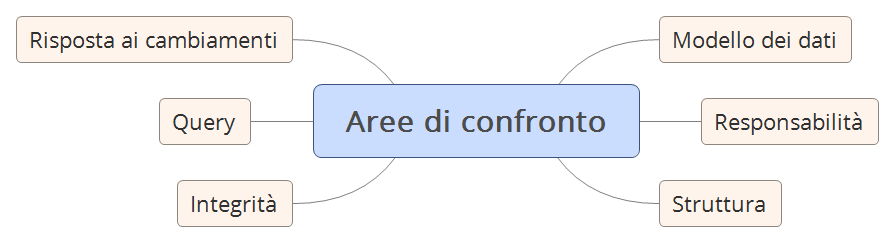
\includegraphics[scale=0.4]{immagini/aree-confronto}
%			\caption{Aree di confronto tra RDBMS e JCR.}
%		\end{figure}
%		
%		\begin{enumerate}
%			\item \textbf{Modello dei dati} \\
%			Con \jquote{modello dei dati} intendiamo il modo con cui i dati vengono organizzati, acceduti e messi in relazione tra di loro.
%			\paragraph{RDBMS} 
%			Il modello relazionale si basa sulla teoria degli insiemi e sulla definizione matematica di relazione, che ricordiamo essere un sottoinsieme del prodotto cartesiano tra \textit{n} insiemi. Dato che ognuno di questi dev'essere distinguibile dagli altri, ogni insieme è definito come dominio. Ad esempio, facendo riferimento alla tabella sottostante, i domini sono quello dei nomi (N), cognomi (C) ed età (E). 
%			
%			\begin{figure}[H]
%				\centering
%				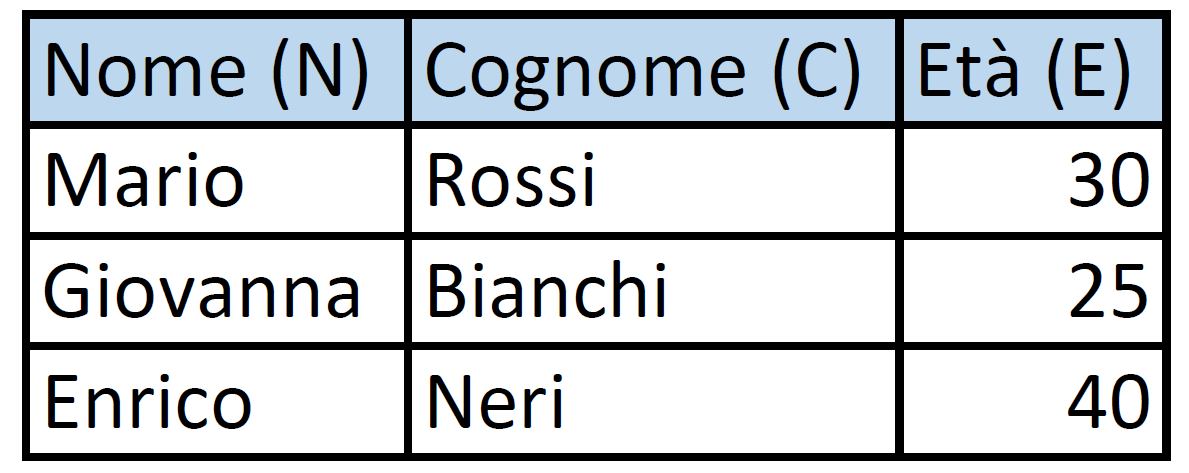
\includegraphics[scale=0.2]{immagini/modello-r}
%				\caption{Tabella che rappresenta una persona (\url{https://goo.gl/ngzgKt}).}
%			\end{figure}
%		
%			La definizione di relazione non implica la possibilità di creare associazioni tra le relazioni. Per fare questo, è necessario utilizzare l'algebra relazionale. 
%			
%			\paragraph{JCR} 
%			Il modello JCR si basa principalmente su una struttura ad albero, unendo le caratteristiche dei modelli gerarchici a quelle dei modelli a rete. Il risultato è una struttura ad albero che permette la connessione dei nodi orizzontalmente.
%			
%					\begin{figure}[H]
%						\centering
%						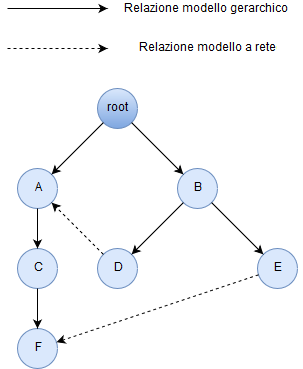
\includegraphics[scale=0.5]{immagini/modello-j}
%						\caption{Unione del modello a rete con il modello gerarchico (\url{https://goo.gl/ngzgKt}).}
%					\end{figure}
%				
%			\item \textbf{Responsabilità} \\
%			Quando si tratta di \textit{database} e persistenza dei dati, generalmente possono essere identificati tre ruoli principali:
%			\begin{itemize}
%				\item Il \textbf{\textit{database administrator} (DBA)}, che mantiene il \textit{database} in uno stato utilizzabile eseguendo attività di installazione, configurazione, \textit{backup} e \textit{data recovery}.
%				\item L'\textbf{\textit{application programmer}}, che scrive \textit{software} che accede al \textit{database}.
%				\item L'\textbf{utente}, che utilizza il \textit{software} per leggere, scrivere e modificare i dati nel \textit{database}.
%			\end{itemize}
%			I due modelli si differenziano anche sotto il punto di vista dei ruoli. Più precisamente, cambiano le responsabilità e i campi di interesse di ogni ruolo.
%			
%			
%			I campi di interesse presi in esame sono:
%			\begin{itemize}
%				\item \textbf{Contenuto}: tutti i dati inclusi nel \textit{database}.
%				\item \textbf{Struttura}: il modo con cui i dati sono suddivisi.
%				\item \textbf{Integrità}: lo stato di completezza dei dati.
%				\item \textbf{Coerenza}: la relazione ordinata, logica e consistente delle parti.
%			\end{itemize}
%			
%			
%			\paragraph{RDBMS} 
%				Nel modello relazionale generalmente è il DBA ad avere il controllo sulla struttura. L'\textit{application programmer} solitamente ha un qualche tipo di influenza sulle decisioni prese in questo campo, ma la decisione finale spetta al DBA. L'utente non ha alcuna responsabilità per quanto riguarda la struttura e può solo interagire con il \textit{database} tramite le operazioni fornite dal \textit{software}.
%				
%				\begin{figure}[H]
%					\centering
%					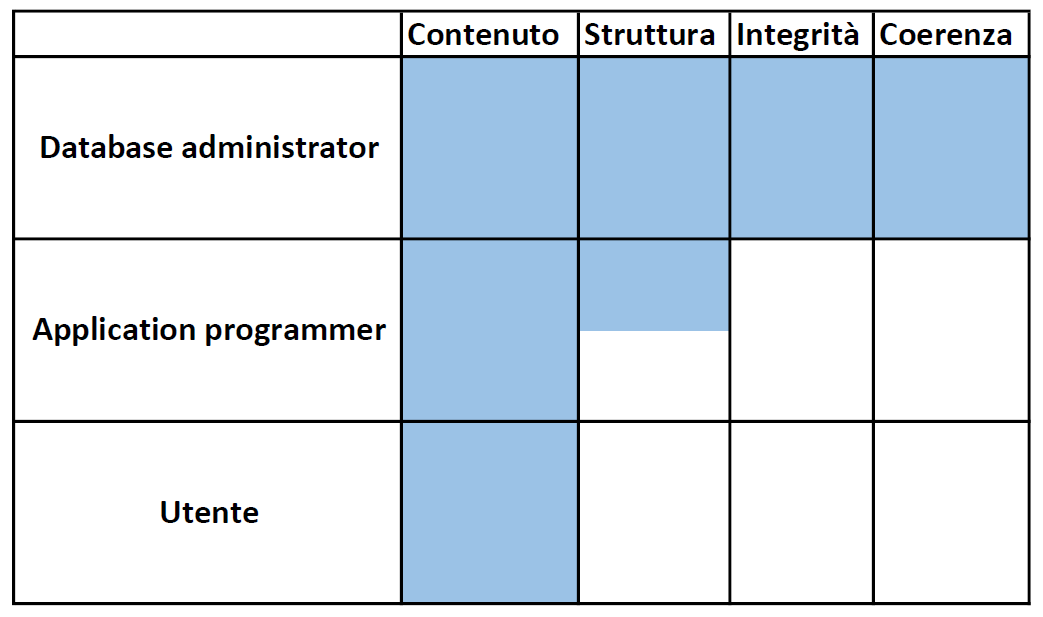
\includegraphics[scale=0.4]{immagini/ruoli-r}
%					\caption{Responsabilità dei ruoli in RDBMS (\url{https://goo.gl/ngzgKt}).}
%				\end{figure}
%			
%			
%			\paragraph{JCR} 
%				Nel modello JCR invece la struttura è responsabilità di tutti e tre i ruoli. Infatti, il controllo sulla struttura è più incentrato verso l'\textit{application programmer} e l'utente, riducendo di fatto le responsabilità del DBA in questo campo.
%				
%				
%				Uno dei vantaggi principali di questo approccio è che solitamente il ruolo di \textit{application programmer} è più vicino all'utente finale rispetto al DBA, quindi una collaborazione tra questi due ruoli per la definizione della struttura è solitamente più efficace.
%				
%				
%				È anche possibile costruire \textit{software} che permettono al solo utente finale di definire la struttura, aggiungendo attributi ai dati a tempo di esecuzione, sottostando ai vincoli definiti dal DBA e dall'\textit{application programmer}.
%				
%				\begin{figure}[H]
%					\centering
%					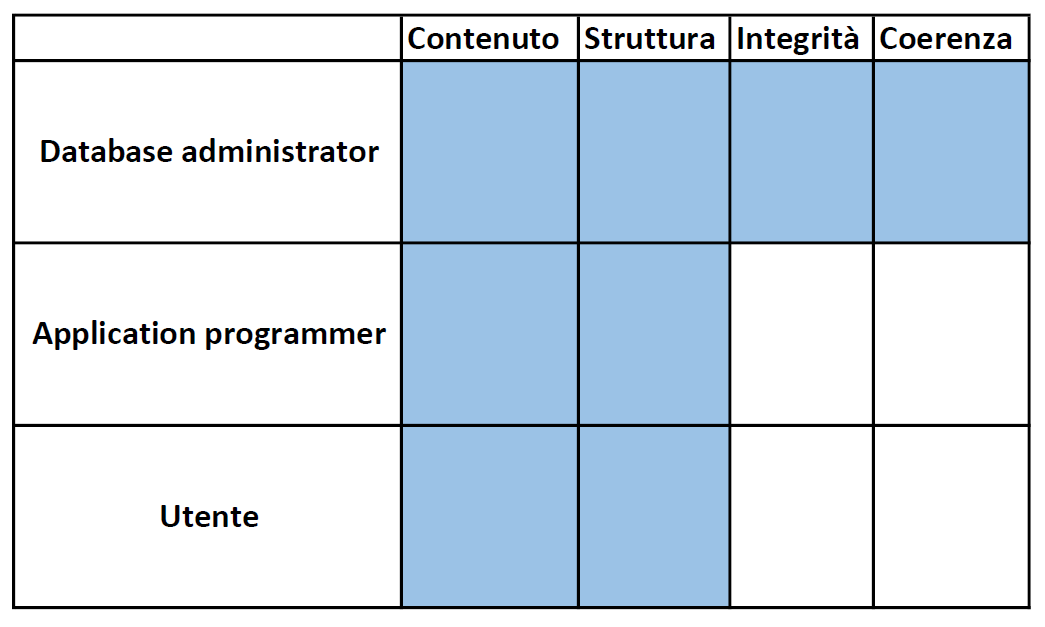
\includegraphics[scale=0.4]{immagini/ruoli-j}
%					\caption{Responsabilità dei ruoli in JCR (\url{https://goo.gl/ngzgKt}).}
%				\end{figure}
%				
%				\item \textbf{Struttura} \\
%					Con \jquote{struttura} intendiamo il modo con cui i dati sono suddivisi e a quali costrizioni essi sono sottoposti. 
%					
%					
%					Le differenze in termini di struttura rendono i due modelli diametralmente opposti, con vantaggi e svantaggi in entrambi gli approcci.
%					
%					\paragraph{RDBMS} 
%						Nel modello RDBMS, i dati sono guidati dalla struttura. Un dato, per essere istanziato, ha bisogno che la struttura sia completamente definita. Questo modello si basa sull'assunzione che dati e struttura siano sempre completamente separati e indipendenti, ma nella realtà quest'assunzione non è sempre valida. Come esposto precedentemente, ci sono casi d'uso in cui la struttura del dato cambia nel tempo, portando all'aggiunta di nuovi campi o ad un'intera riprogettazione nei casi più sfortunati.
%					
%					\paragraph{JCR} 
%						In JCR non è richiesta la definizione di alcuna struttura per istanziare i dati. Nodi, attributi e valori possono essere creati senza nessun prerequisito. Infatti, la struttura emerge con l'inserimento dei dati. Con il modello JCR non è più necessario definire tutti i possibili attributi al momento della creazione di un tipo di dato, garantendo una maggiore flessibilità ed estendibilità.
%						
%				
%				
%				\item \textbf{Integrità} \\
%					L'integrità di un \textit{database} indica l'impossibilità di distruzioni e alterazioni dei dati, siano esse accidentali o intenzionali. Questa caratteristica è implementata in diversi modi a seconda del modello.
%					
%					\paragraph{RDBMS} 
%						Il modello relazionale adotta una strategia simile ad una \textit{white list}, ovvero i dati possono essere salvati solo se è definita una struttura. È quindi quest'ultima che garantisce buona parte dell'integrità, ad esempio attraverso i vincoli di dominio.
%					
%					
%					\paragraph{JCR} 
%						In opposizione al modello RDBMS, JCR si basa su un approccio a \textit{black list}. Un nodo generico del \textit{Content Repository} può avere qualunque nodo figlio e qualsiasi proprietà, senza vincoli su tipi e valori.
%						
%						
%						Eventuali vincoli possono essere imposti assegnando ai nodi dei tipi. Un tipo di nodo descrive vincoli sul tipo dei nodi figli o sui valori delle proprietà che il nodo stesso può avere. Assegnando un tipo anche ai nodi figli e continuando a procedere in questo modo è possibile imporre sempre più limiti alla struttura.
%						
%				\item \textbf{\textit{Query}} \\
%					Anche il tipo e la potenza delle \textit{query} differenzia i due modelli.
%				
%					\paragraph{RDBMS} 
%						Data la definizione di relazione, il modello RDBMS si basa sull'algebra relazionale per la definizioni delle operazioni di base. Il vantaggio di questo modello è che sia l'\textit{input} che l'\textit{output} delle operazioni sono relazioni. È quindi possibile concatenare espressioni complesse senza troppe difficoltà. Inoltre, la maggior parte dei linguaggi di \textit{query} fornisce anche la possibilità di effettuare cambiamenti sequenziali al risultato di una \textit{query}.
%					
%					
%					\paragraph{JCR} 
%						Nel JCR è necessario utilizzare un modello di \textit{query} astratto per effettuare operazioni. Questo modello astratto serve a mappare il modello JCR con le nozioni di relazione, domini, tuple e attributi tipiche del modello relazionale.
%						
%						
%						Uno dei principali svantaggi è che, con l'implementazione JCR di \textit{default}, non è possibile effettuare cambiamenti sequenziali con una \textit{query}.
%					
%					
%						Nel complesso, JCR offre un supporto più limitato rispetto al modello relazionale per quanto riguarda le \textit{query}, ma ha vantaggi prestazionali nell'esecuzione di ricerche \gls{fulltext}.
%					
%				\item \textbf{Risposta ai cambiamenti} \\
%					Nonostante un'analisi dei requisiti svolta in maniera impeccabile, è possibile che nuovi requisiti emergano dopo che l'architettura di un sistema è già stata definita. Un modello di sviluppo non strettamente sequenziale, come ad esempio quello incrementale, permette solitamente di soddisfare i nuovi requisiti senza dover riprogettare interamente il sistema. Tuttavia, un impatto a livello di architettura è spesso inevitabile e comporta dei costi. Per diminuire questi costi, è preferibile adottare un modello dei dati che riesca ad accettare i cambiamenti in maniera trasparente.
%					
%					\paragraph{RDBMS} 
%						Nel modello relazionale, quasi tutti i cambiamenti architetturali richiedono un cambiamento a livello di logica dei dati. Questo modello non è quindi molto adatto a casi in cui sono necessari molti cambiamenti.
%					
%					
%					\paragraph{JCR} 
%						Dato che un'architettura basata sul modello JCR è molto lasca, è possibile aggiungere nuovi campi dati (e quindi soddisfare i requisiti che lo richiedono) senza modificare il livello di logica dei dati. Con JCR si ha quindi un disaccoppiamento molto forte tra dati e logica dell'applicazione. 
%						Data questa caratteristica, l'aggiunta di eventuali campi dati impatterà solo il livello di logica dell'applicazione e di interfaccia. Alcuni \gls{framework} si occupano di un ulteriore disaccoppiamento tra logica e interfaccia operando in maniera simile. Questa combinazione genera un sistema che risponde ai cambiamenti in modo estremamente dinamico e con costi contenuti.
%		\end{enumerate}
%				
%
%		
%	\subsection{Obiettivi}
%		\label{sec:obiettivi}
%	
%	Dopo vari incontri con il \textit{tutor} aziendale, abbiamo definito gli obiettivi da raggiungere, suddividendoli in obbligatori, desiderabili e facoltativi.
%	
%	
%	A grandi linee, nelle trecentoventi ore previste dallo \textit{stage} l'azienda si aspettava:
%	\begin{itemize}
%		\item Uno studio e la produzione di documentazione sulle differenze tra \textit{database} relazionale e \textit{Content Repository}.
%		\item Uno studio e la produzione di documentazione sugli \textit{standard} JSR 170 e JSR 283, rispettivamente Java Content Repository 1.0 e 2.0.
%		\item La produzione di esempi di codice sorgente riguardanti l'utilizzo della libreria \gls{jackrabbit}.
%		\item La realizzazione di un prototipo che permettesse operazioni di aggiunta, visualizzazione, modifica e rimozione di prodotti commerciali e dei loro attributi
%	\end{itemize}
%
%	Con il \textit{tutor} abbiamo discusso anche dell'eventuale possibilità dello studio e dell'implementazione di soluzioni distribuite, ma dato il tempo limitato a disposizione e la corposità delle librerie da apprendere abbiamo deciso di non inserire questa richiesta negli obiettivi.
%	
%	
%	A seguire includo una lista dettagliata degli obiettivi suddivisi per importanza.
%	
%	\begin{table}[H]
%		\begin{tabularx}{\textwidth}{| X |}
%			\Xhline{2\arrayrulewidth}
%			\textbf{Obiettivi obbligatori} \\
%			\Xhline{2\arrayrulewidth}
%			Studio e documentazione sulle differenze tra \textit{database} relazionale e \textit{Content Repository} \\
%			\hline
%			Studio e documentazione sulla storia di \textit{Content Repository} \\
%			\hline
%			Studio di JSR 170 e JSR283: Content Repository for Java (JCR), con produzione di codice e documentazione \\
%			\hline
%			Studio e documentazione della struttura di JCR \\
%			\hline
%			Studio e documentazione della definizione di nodo \\
%			\hline
%			Studio e documentazione riguardo aggiunta, rimozione e modifica di proprietà di un nodo \\
%			\hline
%			Studio e documentazione riguardo l'aggiunta e la rimozione di tipologie di nodo \\
%			\hline
%			Studio e documentazione riguardo la referenziazione di elementi \\
%			\hline
%			Studio e documentazione riguardo l'esecuzione di \textit{query} utilizzando XPath e JCR-SQL2 \\
%			\hline
%			Studio e documentazione riguardo l'indicizzazione \\
%			\hline
%			Progettazione di un prototipo di applicazione che gestisca le informazioni di prodotti commerciali \\
%			\hline
%			Realizzazione di un prototipo di applicazione che gestisca le informazioni di prodotti commerciali \\
%			\Xhline{2\arrayrulewidth}
%			\textbf{Obiettivi desiderabili} \\
%			\Xhline{2\arrayrulewidth}
%			Realizzazione della \gls{gui} del prototipo \\
%			\Xhline{2\arrayrulewidth}
%			\textbf{Obiettivi facoltativi} \\
%			\Xhline{2\arrayrulewidth}
%			Studio e documentazione riguardo i \textit{workspace} multipli \\
%			\hline
%		\end{tabularx}
%		\caption{Obiettivi del progetto}
%	\end{table}
%	
%	\subsection{Vincoli}
%		\begin{figure}[H]
%		\centering
%			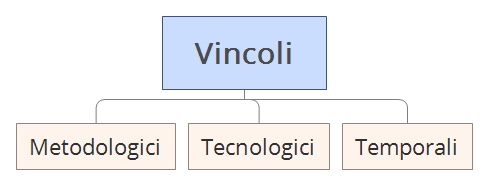
\includegraphics[scale=0.5]{immagini/vincoli}
%			\caption{Vincoli del progetto}
%		\end{figure}
%	
%	\subsubsection*{Metodologici}
%		La prima tipologia di vincoli a cui il progetto era sottoposto erano i vincoli metodologici.
%		
%		
%		Con il \textit{tutor} aziendale abbiamo stabilito che il lavoro doveva essere svolto presso la sede aziendale, per avere miglior approccio e comunicazione con il \textit{tutor} stesso e gli altri colleghi. L'azienda ha posto questo vincolo anche per cercare raggiungere l'obiettivo di prospettiva di assunzione descritto nella sezione \ref{sec:motivazioni_aziendali}.
%		
%		
%		Un altro vincolo stabilito riguardava l'interazione con il \textit{tutor} e la richiesta di informazioni tecniche ai colleghi. Dati i frequenti impegni del \textit{tutor}, nel caso di necessità di informazioni tecniche avrei dovuto chiedere ai colleghi d'ufficio facenti parte del \textit{team} Java 3, senza però abusare di tale possibilità. Uno degli obiettivi che l'azienda ha cercato di raggiungere con questo vincolo è quello di migliorare le mie capacità di \textit{problem solving} e di lavoro in autonomia, insegnandomi a riconoscere i problemi risolvibili da me e quelli che invece necessitano di personale più esperto. I rapporti con il \textit{tutor} si sarebbero dovuti limitare a richieste riguardo i requisiti e a revisioni periodiche per valutare i risultati raggiunti.
%		
%	\subsubsection*{Tecnologici}
%		\label{sec:vincoli-tecnologici}
%		Gli unici vincoli tecnologici imposti dall'azienda riguardavano l'implementazione di esempi di codice e di un prototipo basato sulla libreria Jackrabbit, utilizzando quindi il linguaggio Java.
%		
%		
%		Per quanto riguarda il versionamento, IBC ha predisposto un \textit{repository} SVN su cui avrei dovuto effettuare i \textit{commit} di codice e documentazione.
%		
%		
%		Non abbiamo fissato vincoli stretti riguardo la gestione della configurazione, anche se il \textit{tutor} mi ha fortemente consigliato di utilizzare Maven, data l'esperienza positiva che l'azienda ha avuto con tale strumento.
%		
%		
%		La scelta di eventuali \textit{framework} per l'implementazione dell'interfaccia grafica del prototipo era libera, a patto che fosse possibile l'interfacciamento con il JCR offerto da Jackrabbit. Questo mi ha portato a dover effettuare una scelta:
%		\begin{itemize}
%			\item La prima opzione che ho considerato è stato l'utilizzo del linguaggio PHP, da me già conosciuto. Ho presto realizzato che per percorrere questa strada avrei dovuto utilizzare la libreria Jackalope, che fornisce un'implementazione di JCR accessibile tramite API PHP. Nonostante la presenza di Jackalope-Jackrabbit, un'implementazione basata sul JCR fornito da \gls{jackrabbit}, ho trovato questa soluzione troppo complicata e scarsamente documentata.
%			\item La seconda opzione che ho considerato è stato JavaServer Faces (JSF), un \textit{framework} Java basato sul \textit{design pattern} MVC per lo sviluppo di applicazioni \textit{web}. Dopo aver letto varie opinioni \textit{online}, ho scartato questa scelta in quanto risulta essere molto complicata. Uno dei motivi principali di questa complessità è, come citato da ThoughtWorks nell'articolo raggiungibile al link \url{https://goo.gl/dfxpaC}, \jquote{pensiamo che [JSF] sia imperfetto in quanto tenta di astrarre troppo l'HTML, il CSS e l'HTTP}.
%			\item La terza opzione, quella da me scelta, è stato Apache Wicket, anch'esso un \textit{framework} Java che utilizza MVC con la caratteristica aggiuntiva di essere basato su componenti. Questa caratteristica, unita al fatto che Wicket permetteva l'interfacciamento senza alcuna complicazione al JCR e che era utilizzato anche da IBC, mi hanno portato a preferirlo alle altre tecnologie.
%		\end{itemize}
%		Alla luce di questa e altre decisioni, includo una tabella che elenca le tecnologie utilizzate durante il progetto.
%		
%		\begin{table}[H]
%			\centering
%			\begin{tabularx}{\textwidth}{|X | X | X |}
%				\hline
%				\rowcolor{lightgray}
%			  \textbf{Documentazione} & 	\textbf{{Config.} e \mbox{versionamento}}  &  \textbf{Sviluppo} \\
%				\hline
%				 LibreOffice & Maven & Eclipse \\
%				\hline
%				 & SVN & Jackrabbit \\
%				\hline
%				 & Tomcat & Wicket \\
%				\hline
%				& & Wicket-Bootstrap \\
%				\hline
%				& & JUnit \\
%				\hline
%			\end{tabularx}
%			\caption{Principali tecnologie utilizzate nel progetto.}
%		\end{table}
%	
%	\subsubsection*{Temporali}
%		Per quanto riguarda i vincoli temporali, gli orari di lavoro erano gli stessi del personale IBC, ovvero dal Lunedì al Venerdì con orario dalle 8:30 alle 12:30 e dalle 14:00 alle 18:00. L'azienda non ha richiesto moduli o procedure particolari per l'assenza da lavoro o la variazione di orario per motivi universitari, tranne la comunicazione a voce al \textit{tutor} o ad un collega.
%		
%		
%	\subsection{Pianificazione del lavoro}
%		La pianificazione del lavoro ha dovuto tener conto dei vincoli temporali esposti nella sezione precedente.
%		
%		
%		Ho pianificato lo svolgimento delle attività in otto settimane lavorative da quaranta ore ciascuna, come mostrato nel Gantt sottostante.
%			\begin{figure}[H]
%				\centering
%				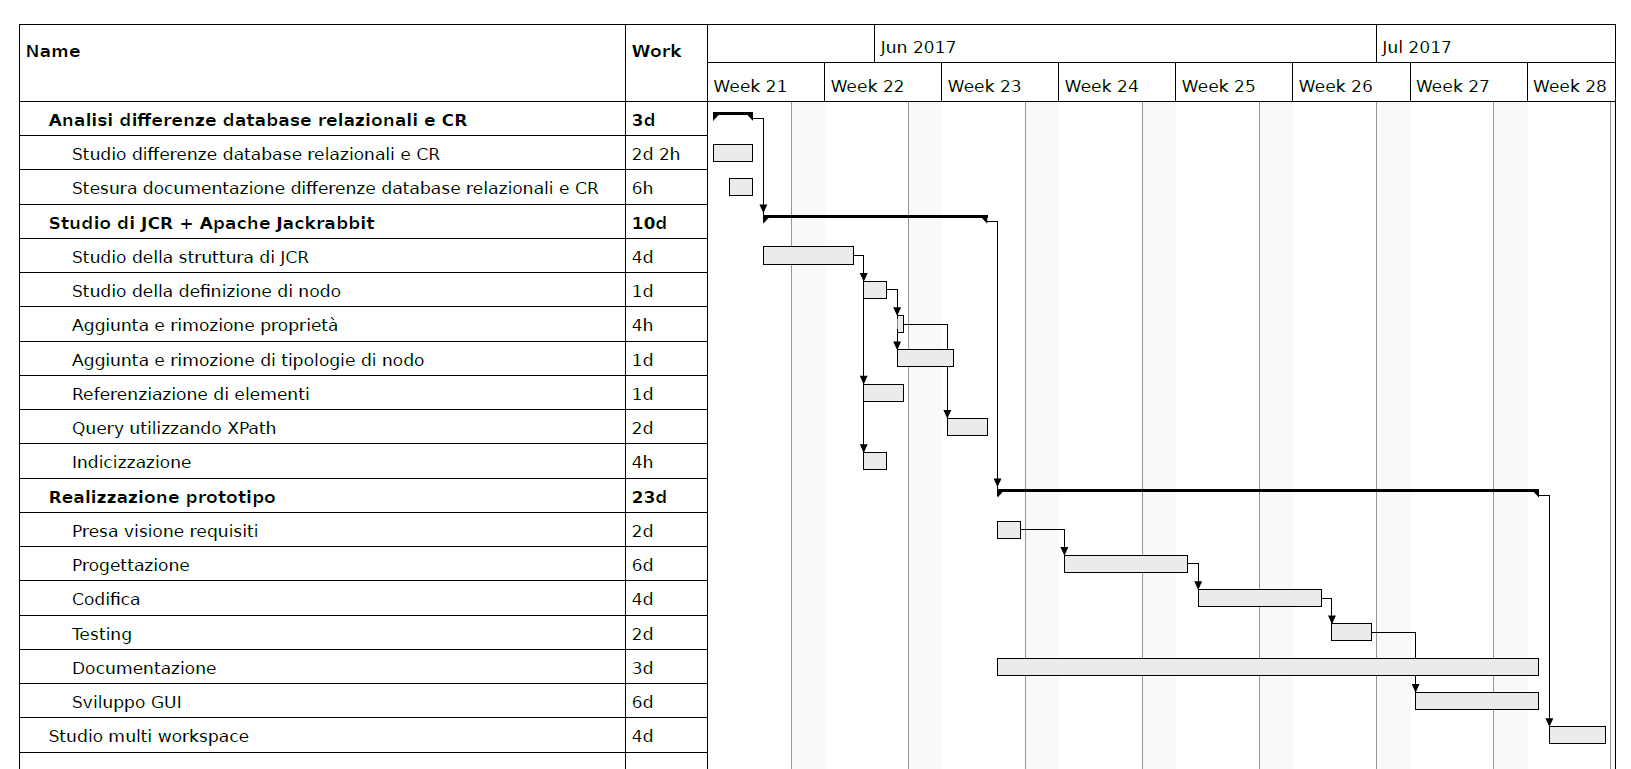
\includegraphics[width=\textwidth]{immagini/gantt-pianificazione}
%				\caption{Pianificazione temporale.}
%			\end{figure}
%		
%		Durante lo svolgimento iniziale delle attività di analisi e studio ho seguito il piano, ma durante la realizzazione del prototipo non ho rispettato la netta sequenzialità tra realizzazione del prototipo e sviluppo della GUI. Il motivo di questa decisione è dovuto al fatto che ho deciso di raggiungere l'obiettivo desiderabile stabilito dal piano di lavoro. Ho avuto quindi la necessità di iniziare ad apprendere il \textit{framework} scelto per l'interfaccia al più presto, portandomi a svolgere le attività di realizzazione della logica del prototipo e della parte grafica in parallelo.
%
%		Tenendo conto di questo punto, il reale svolgimento delle attività è stato il seguente.
%		
%		\begin{figure}[H]
%			\centering
%			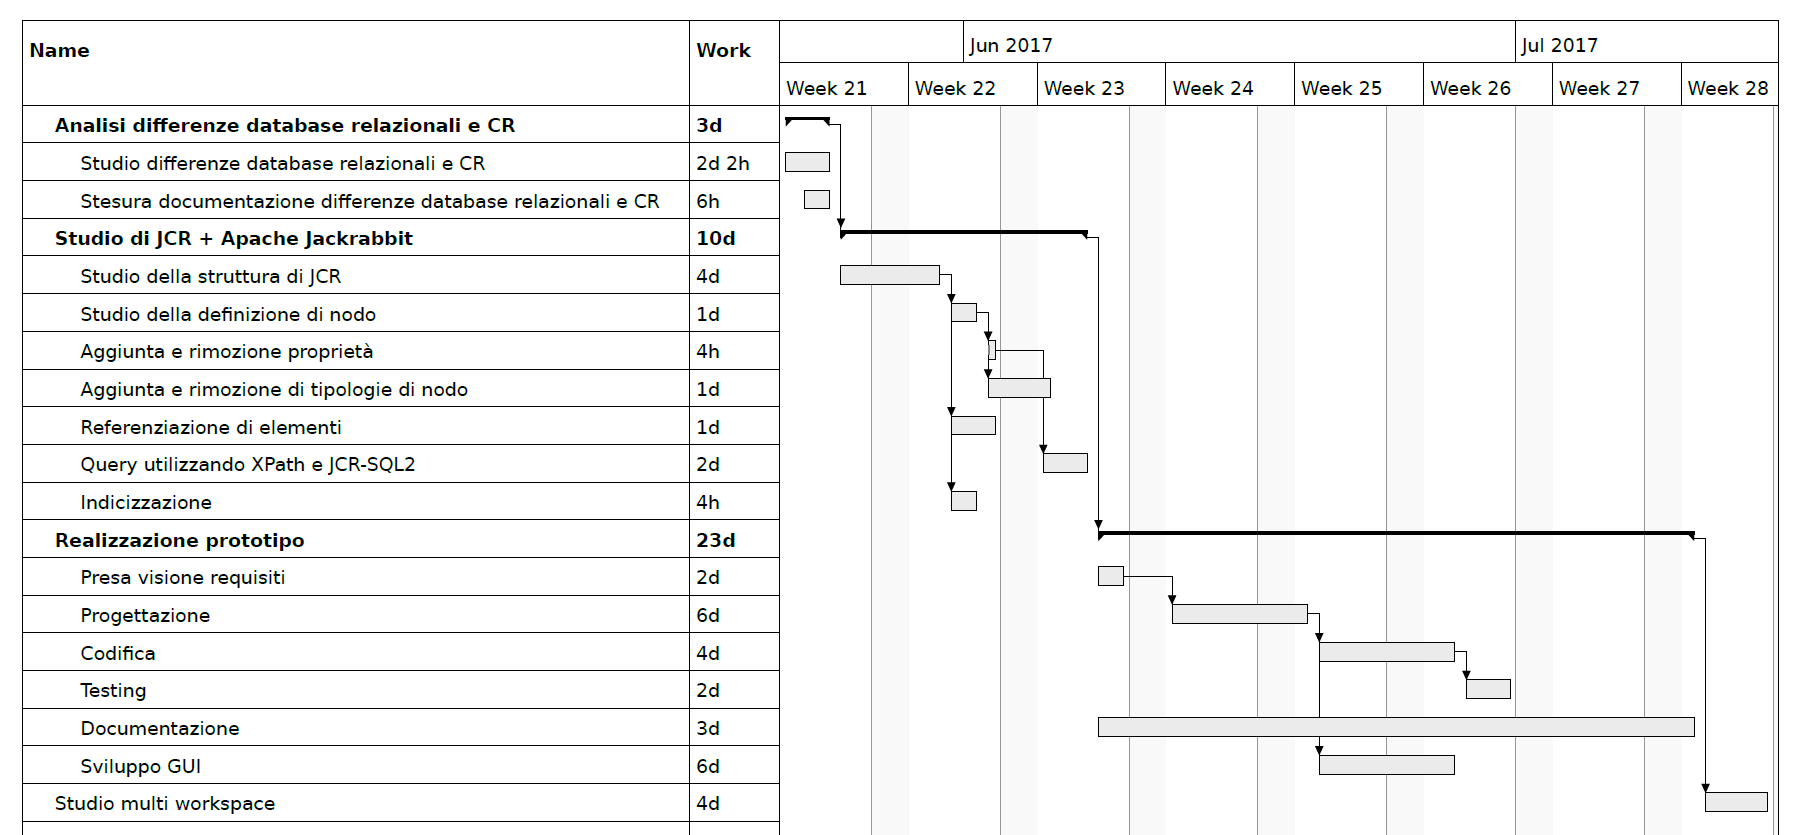
\includegraphics[width=\textwidth]{immagini/gantt-consuntivo}
%			\caption{Svolgimento attività.}
%		\end{figure}
%		
%
%\section{\textit{Stage} in IBC: motivazioni personali}
%	\label{sec:motivazioni_personali}
%	Durante la partecipazione a StageIt ho sostenuto colloqui con undici aziende. La mia scelta è ricaduta su IBC per una serie di motivi suddivisibili in tre tipologie: economici e logistici, professionali, personali.
%	
%	\subsubsection*{Economici e logistici}
%		\begin{itemize}
%			\item L'azienda, al contrario di molte altre, offriva un rimborso spese. Personalmente lo considero come un modo di riconoscere del valore nel lavoro svolto dallo stagista. Inoltre, la gratificazione ricevuta da questo riconoscimento è un buon punto di partenza per un rapporto che potrebbe continuare dopo la fine dello \textit{stage}.
%			\item Il posizionamento del luogo di lavoro, situato a dieci minuti da casa e vicino a Padova, era ideale per permettermi di raggiungere in breve tempo la sede dell'università. Infatti, data la necessità di terminare il progetto didattico di \gls{swe}, ho dovuto presenziare ad alcuni incontri con i miei compagni di progetto dopo l'orario di lavoro. Un'azienda situata più lontano non mi avrebbe permesso tale flessibilità.
%		\end{itemize}
%	
%	\subsubsection*{Professionali}
%		\begin{itemize}
%			\item IBC è un'azienda che non si occupa solamente di consulenza, ma produce anche \textit{software} proprio. Svolgere lo \textit{stage} presso IBC mi ha permesso di essere immerso in un ambiente che unisce entrambe le realtà.
%			\item Data la diffusione del linguaggio Java in ambito aziendale, ho valutato positivamente un'esperienza in una realtà che, oltre ad usare tale linguaggio, produce applicazioni che si basano su \gls{javaee}.
%		\end{itemize}
%	
%	\subsubsection*{Personali}
%	\begin{itemize}
%		\item Con questo \textit{stage} ho voluto valutare se l'impiego presso un'azienda che produce \textit{software} fosse adatto a me. Inoltre, dato che questa sarebbe stata la mia prima esperienza lavorativa, mi sono posto come obiettivo quello di rapportarmi con il personale esperto per avere consigli ed informazioni su come gestire un lavoro in campo informatico.
%	\end{itemize}
%
%%**************************************************************
%%\chapter{L'azienda}
%%\label{cap:lazienda}
%%%**************************************************************
%%
%%Introduzione al contesto applicativo.\\
%%
%%\noindent Esempio di utilizzo di un termine nel glossario \\
%%\gls{api}. \\
%%
%%\noindent Esempio di citazione in linea \\
%%\cite{site:agile-manifesto}. \\
%%
%%\noindent Esempio di citazione nel pie' di pagina \\
%%citazione\footcite{womak:lean-thinking} \\
%%
%%%**************************************************************
%%\section{L'azienda}
%%
%%Descrizione dell'azienda.
%%
%%%**************************************************************
%%\section{L'idea}
%%
%%Introduzione all'idea dello stage.
%%
%%%**************************************************************
%%\section{Organizzazione del testo}
%%
%%\begin{description}
%%    \item[{\hyperref[cap:processi-metodologie]{Il secondo capitolo}}] descrive ...
%%    
%%    \item[{\hyperref[cap:descrizione-stage]{Il terzo capitolo}}] approfondisce ...
%%    
%%    \item[{\hyperref[cap:analisi-requisiti]{Il quarto capitolo}}] approfondisce ...
%%    
%%    \item[{\hyperref[cap:progettazione-codifica]{Il quinto capitolo}}] approfondisce ...
%%    
%%    \item[{\hyperref[cap:verifica-validazione]{Il sesto capitolo}}] approfondisce ...
%%    
%%    \item[{\hyperref[cap:conclusioni]{Nel settimo capitolo}}] descrive ...
%%\end{description}
%%
%%Riguardo la stesura del testo, relativamente al documento sono state adottate le seguenti convenzioni tipografiche:
%%\begin{itemize}
%%	\item gli acronimi, le abbreviazioni e i termini ambigui o di uso non comune menzionati vengono definiti nel glossario, situato alla fine del presente documento;
%%	\item per la prima occorrenza dei termini riportati nel glossario viene utilizzata la seguente nomenclatura: \emph{parola}\glsfirstoccur;
%%	\item i termini in lingua straniera o facenti parti del gergo tecnico sono evidenziati con il carattere \emph{corsivo}.
%%\end{itemize}